\documentclass[twocolumn]{article}
\usepackage[margin=1.2in]{geometry}

\usepackage[english]{babel}
\usepackage[utf8]{inputenc}
\usepackage{amsmath}
\usepackage{graphicx}
\usepackage{float}
\usepackage[colorinlistoftodos]{todonotes}

\title{A Solution to Drowsy Driving via real-time Image Analysis}

\author{Bruno Peynetti, Michael Nowakowski, \\Baiyu Yang, Yannan Xu}

\date{\today}

\begin{document}
\maketitle



\begin{abstract}
Drowsy Driving is a widespread problem in the United States. It is a known cause of crashes and fatal accidents every year. Nevertheless, identifying drowsiness and acting on it is a challenging task. This paper presents a novel mobile solution in order to identify and act on drowsy drivers. The system aggregates data from a camera mounted on the rear-view mirror which constantly collects information about the driver. We propose an algorithm that analyses the data and determines a threshold of drowsiness based on a variety of factors. The camera-mounted system then transmits that information to a server, from which a smart-phone pulls information and acts on it in order to notify the driver of the danger of falling asleep. 
\end{abstract}

\section{Motivation and Background}
Drowsy Driving is a major problem in the United States. An estimated 1 in 25 adults report having fallen asleep while driving in the previous 30 days. The National Highway Traffic Safety Administration "conservatively estimates that 100,000 police-reported crashes are direct result of driver fatigue each year. This results in at least 1,550 deaths and \$12.5 billion in monetary losses. Nevertheless, the unofficial figures, including accidents that are not reported or attributed to other causes, can be much larger.  \\
A target market for blink detection would be drivers who drive for long periods of time in straight, traffic free areas. For example, truck drivers who travel accross the country need to drive for long hours, and risk falling asleep during the drive. Equally likely are passenger bus drivers. There is inherently a larger incentive to keep bus drivers awake since a simple nod could cause a catastrophic crash. \\
We are also motivated to create a system that is light-weight, portable, and easy to adapt to any situation. To this purpose, we considered using the Raspberry Pi 2 mobile computer with an attached camera, as well as an Android smartphone, which is the most popular type of smartphone and easy to develop for. 

\section{Related Work}
Several studies have proposed a range of methods to detect drowsiness and distractability while driving. Some of these results have been applied to commercial products and have started appearing in the market. For example, a study \cite{fusion} had developed a pilot drowsy driving detection system in the car to capture the images of driver's face by a camera and to collect the driver photoplethysmograph by a bio-signal sensor installed on the steering wheel. The system was developed using Android-based smartphone technology to receive sensory data from a video sensor and a bio-signal sensor. Then, it processed the data to determine the driver's state of fatigue. Another study developed a five-layer sensing architecture to collect information related to the driver in real-time. \cite{sultan}. Other studies \cite{driving_manuever} \cite{sleep_depravation} looked into driving maneuvers to build driver behavior models. On the other hand, a study by Pascale \cite{pascale} proposes traffic monitoring sensors deployed along the road in order to improve quality and safety of car mobility and enable short-term traffic predictions, which might in turn be able to predict driver behavior. Many of these studies do not include an alert system but rather look into identifying the drowsy driving. One study by Sun, Zhang, et.al. \cite{smartcar} studied a context-aware smart car which collected and evaluated contextual information about the driving, vehicle, and driving environment. A software platform was built for the context model and its applications. 

\section{System Architecture}
In this section, we focus on describing the layout of the system architecture and the functionality of the system. 
\subsection{Mounted Camera and Image Analysis Unit}
In order to successfully identify driver fatigue using image analysis, a camera has to be placed in the correct location and at the right angle pointed at the driver. A smartphone camera will not always be in the best position, since different users change the location of their smartphone on the dashboard, and many place it at an angle such that a forward-facing camera would not point at the driver. \\
Since our solution relies on being able to detect drowsy driving as quickly and reliable as possible, it is of outmost importance to have the correct camera placement. The camera is to be placed in the bottom left corner of the rearview mirror, providing an almost direct view of the driver without obstructing the view. Figure \ref{fig:camera} shows the positioning of the camera next to the rear-view mirror. The small size of the camera allows for almost no obstruction to the driver's view. 

\begin{figure}[H]
\centering
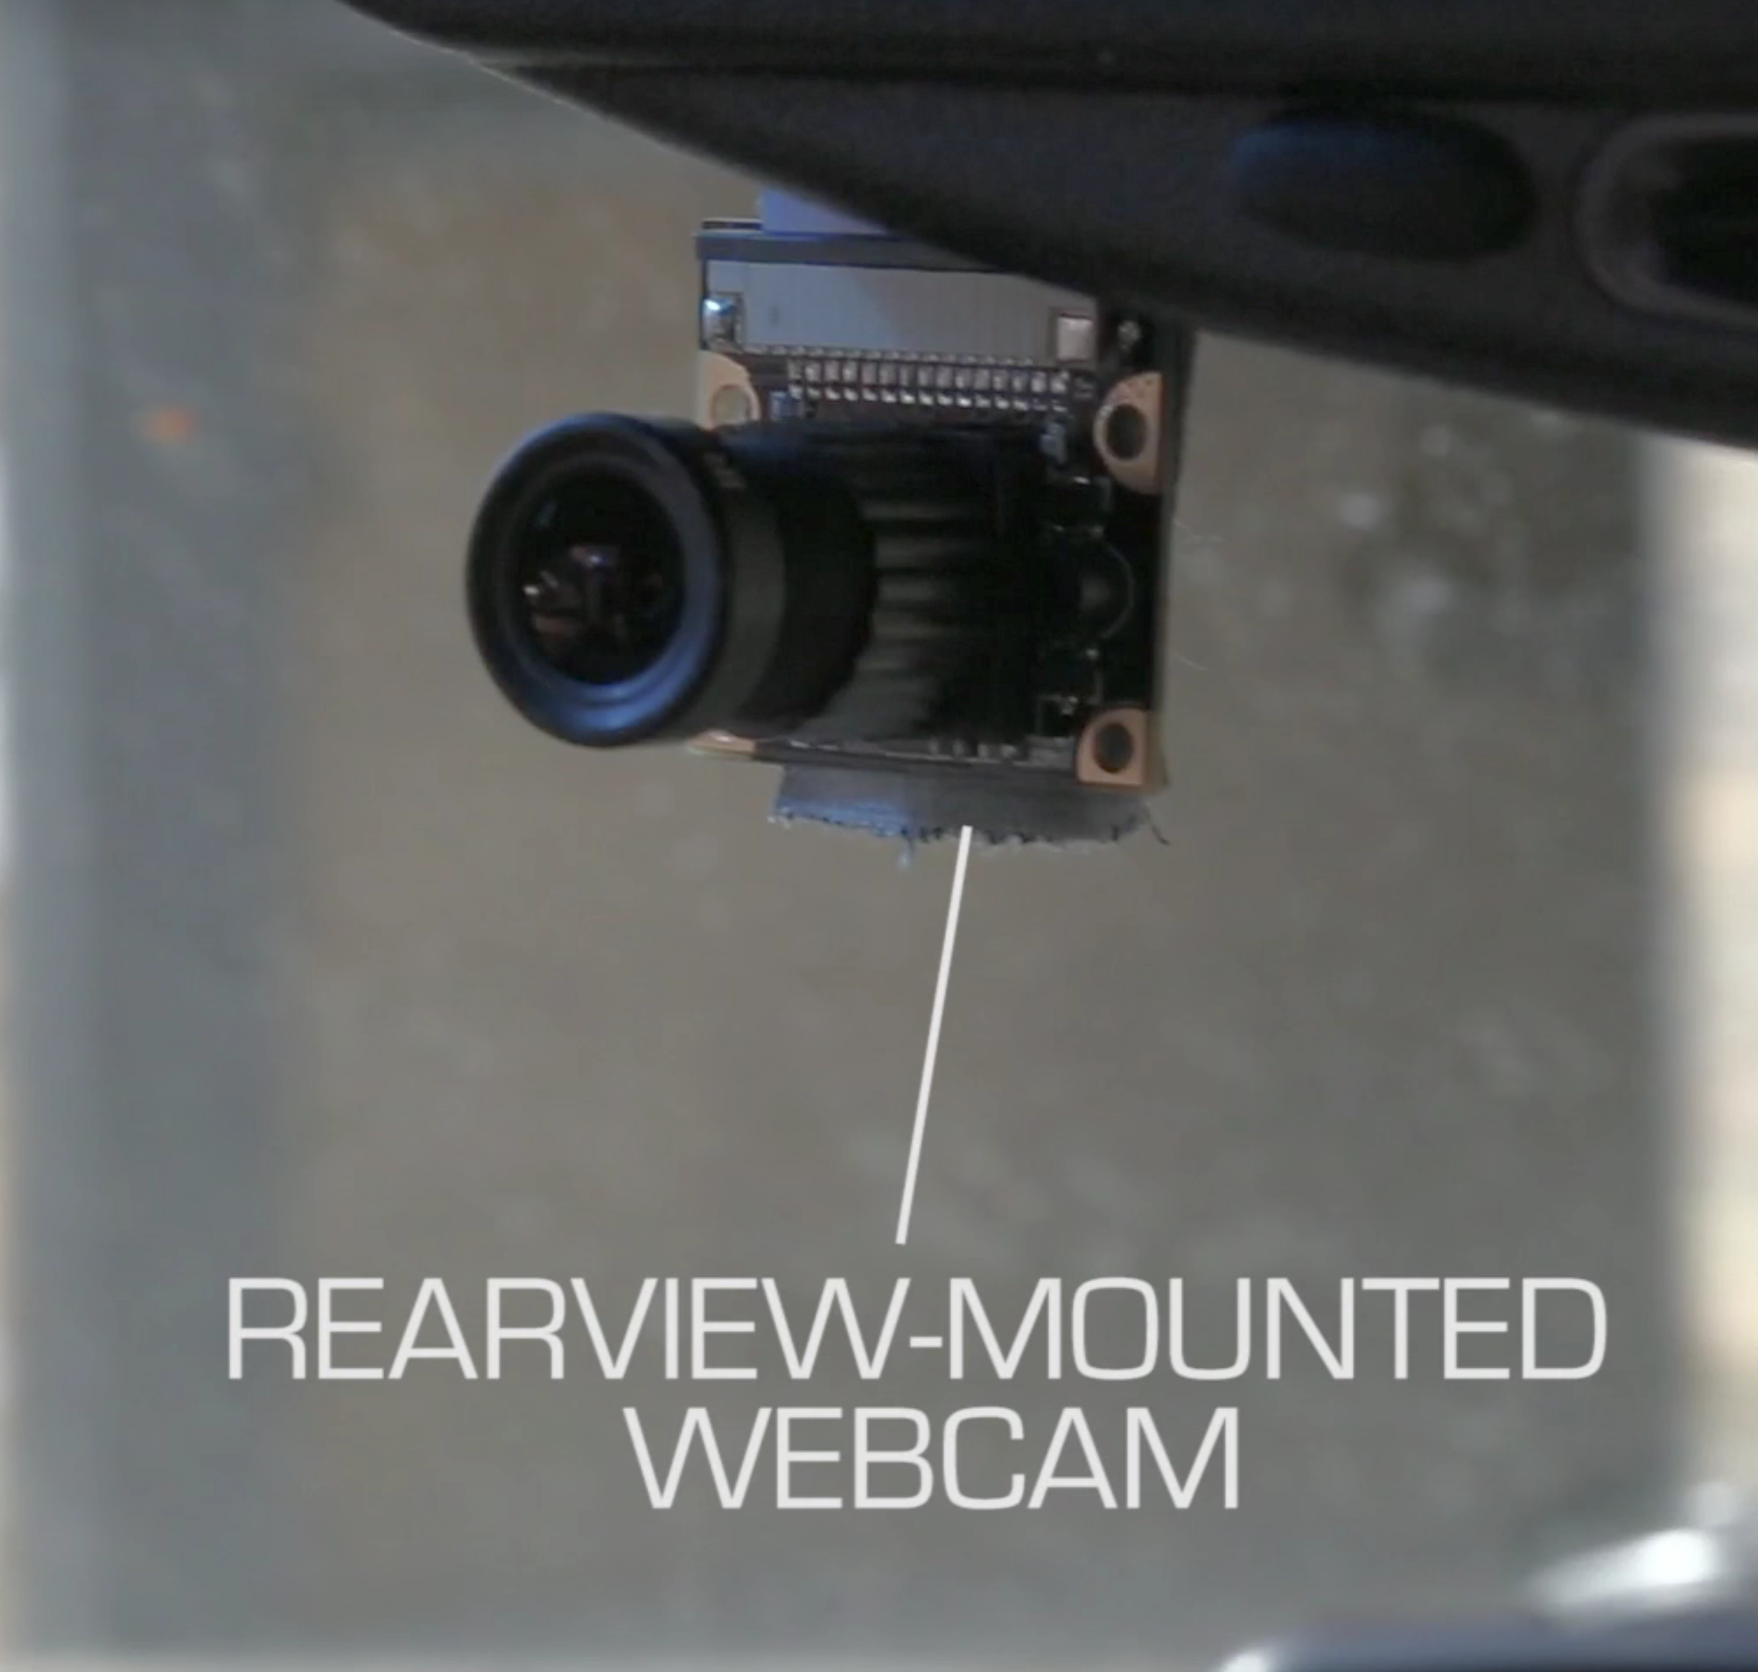
\includegraphics[width=0.8\linewidth]{./camera.png}
\caption{Raspberry Pi Camera }
\label{fig:camera}
\end{figure}

\subsection{Back-end Server}
We chose to use a back-end server to store data and act as the intermediary between the smartphone and the Raspberry Pi (the image analysis unit). After the Raspberry Pi executes the drowsiness detection algorithm, the data is sent to a back-end server where it is stored in a MySQL database. When a smartphone sends a GET request to the server, the server responds with a JSON file containing the latest data and a variable that determines whether the driver is drowsy or not. This implementation allows for multiple users to save and request information simultaneously. In addition, all data is being stored and can be analyzed later to improve the drowsiness detection algorithm's accuracy and performance. The server of choice was a LAMP stack (Apache, PHP and MySQL) in the Cloud9 (c9.io) hosting website. This website has a Virtual Machine enabled with terminal access, as well as text editors and debuggers, which allows for easy and efficient and development. 

\subsection{Smartphone}
The smartphone portion of the app involves an information display feature and an alert feature. A simple Android Application was created in order to interact with the user and propose a quick, safe solution in case drowsiness is detected on the driver. We used a variety of Android and test the app. One of them was a Nexus 5. For internet connection we enabled Wi-fi but a cellular connection would work just as well. Figure \ref{fig:app} shows the landing page of the app. In a full development version, the user would have the ability to login and user-specific features would be enabled (such as destination, prompt alert message, etc)

\begin{figure}[H]
\centering
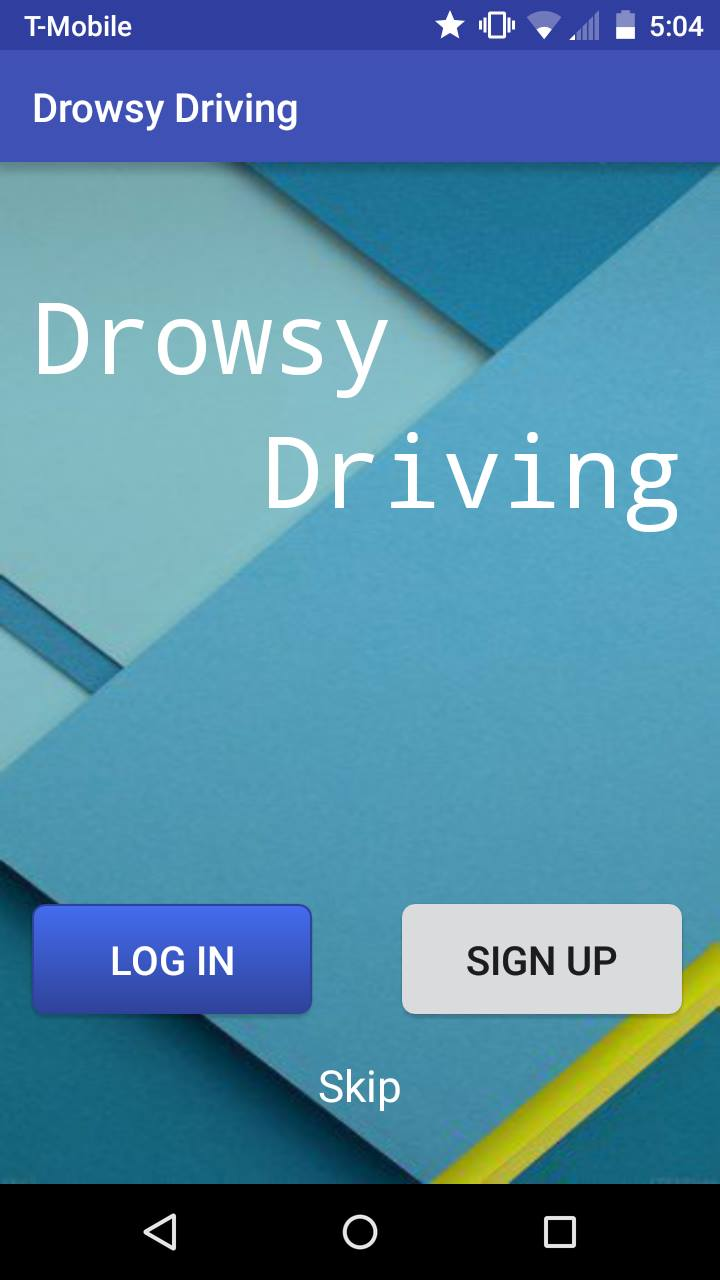
\includegraphics[width=0.6\linewidth]{./logo.jpg}
\caption{App login page }
\label{fig:app}
\end{figure}

\section{Drowsiness Detection Algorithm}
The following section proposes a drowsiness detection algorithm by making use of a variety of classification techniques in order to create a more robust and accurate classifier. Some previous work \cite{pakistan} does not solve the problem by identifying drowsiness, but rather by identifying one of the features of drowsiness such as a closed eye. We chose to focus on 3 features and built a classification algorithm based on these features:
\begin{itemize}
\item Blink rate (blinks per minute)
\item Yawn rate (yawns per minute)
\item Blink length (moving average length of previous blinks)
\end{itemize}
In order to calculate these features, we designed an algorithm that will make use of image recognition analysis in order to detect the face, eyes, and mouth in every frame. Afterwards, information from subsequent frames is fed into the algorithm in order to extract the required features. \\
The flowchart on Figure \ref{fig:drowsy_algo} describes the process to detect drowsiness. The algorithm is attempted with each camera frame, and a different algorithm (discussed later in the section) determines the level of drowsiness. \\


\begin{figure}
\centering
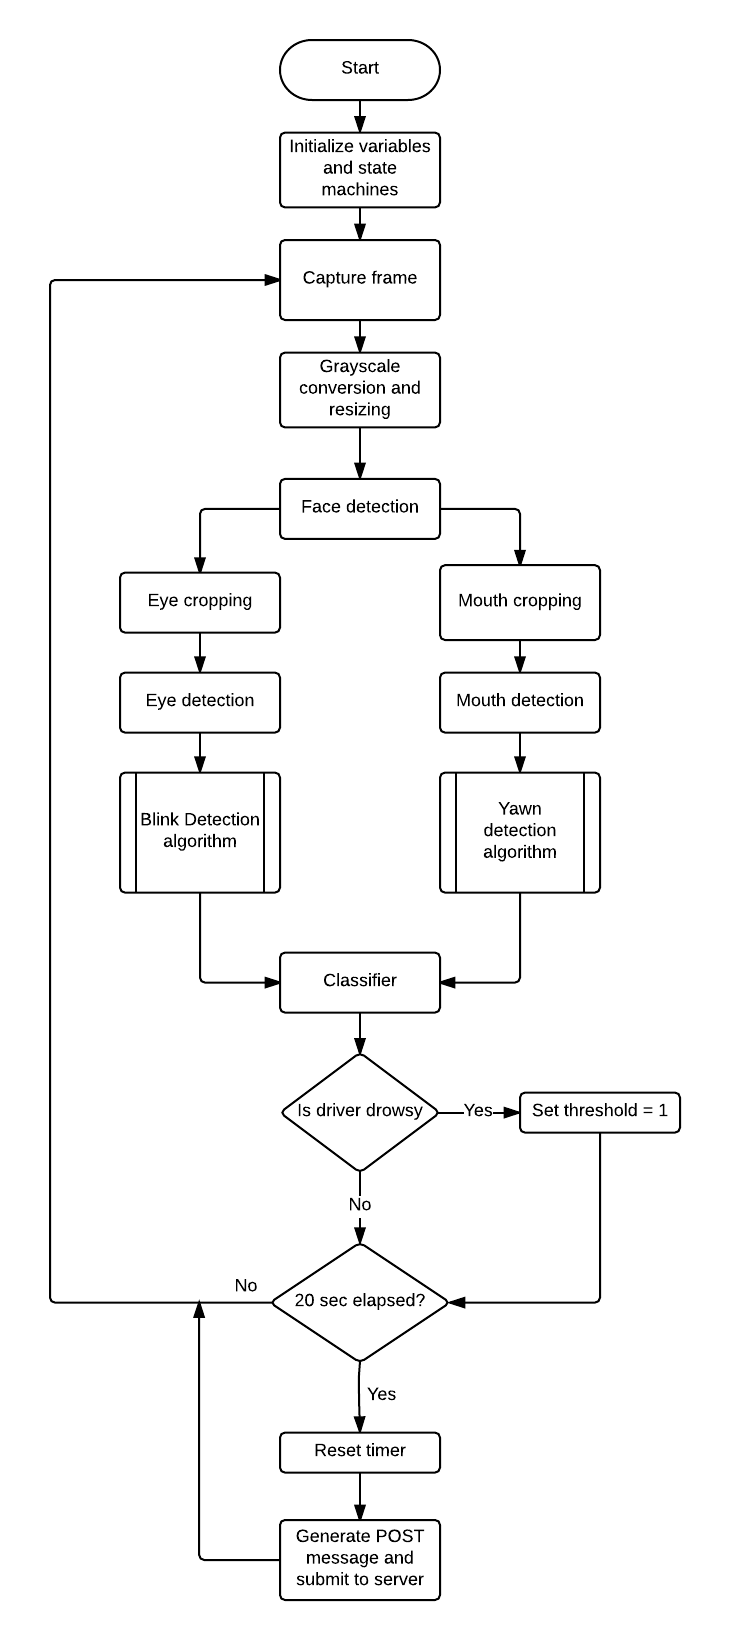
\includegraphics[width=0.95\linewidth]{./flowchart_detection.png}
\caption{Drowsiness Detection Algorithm }
\label{fig:drowsy_algo}
\end{figure}

\begin{figure}
\centering
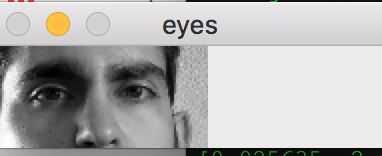
\includegraphics[width=0.25\textwidth]{./eyes.png}
\caption{Eye recognition bounding box }
\label{fig:eyes}
\end{figure}


\subsection{Face Detection}
The first step of the drowsiness detection algorithm is face detection. Since our approach requires image analysis and recognition in each frame, performance is a necessary attribute. Viola and Jones's \cite{viola} algorithm for real-time face detection was deemed appropriate. The algorithm works on the basis of classification based on simple features rather than pixels directly. Viola introduces the concept of an \textbf{Integral image} that contains at location $x,y$ the sum of the pixels above and left of $x,y$. Figure \ref{fig:haar} shows how each rectangular mask and filter compares different intensities of sections of an image in order to create a specific feature. Different combinations of rectangles create tens of thousands of different features. Nevertheless, Viola demonstrated that the correct feature selection (about 200 features) yields a detection rate of about 95\%. In order to decrease the time to process the image, a cascade of weak classifiers is built. Each weak classifier is not able to individually classify the image, but the combination of classifiers is able to discern the correct object. 
\\
\begin{figure}[H]
\centering
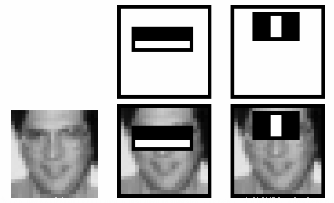
\includegraphics[width=0.25\textwidth]{./haar.png}
\caption{Haar Cascade Classification}
\label{fig:haar}
\end{figure}

The implementation of this classifier was used by means of the Python OpenCV 2.4 library, which is optimized to work as a wrapper for the OpenCV C++ functions, and thus provides a performance similar in its bare-bones Python library as in the C++ implementation. We decided to use the Python version for simplicity of code and development speed. 
\subsection{Eye Detection}
The eye detection algorithm uses a very similar approach to the cascade-based classification that identifies a face. Nevertheless, an eye is harder to recognize and thus easier to miss-classify. As a result, the bounding window on which the eye was searched for was significantly decreased in an effort to achieve higher accuracy and  performance. \\
For an identified face starting at coordinates $(x,y)$ and with a width of $w$ and a height of $h$, the face image can be represented as the following:
$$face = Image[y:y+h,x:x+w]$$ Where $Image$ is the captured frame with a camera. The bounding box for the eye is as following:
$$eye = Image[(y+h/5):(y+h/2),x:(x+w)]$$
The resulting cropped image is shown in Figure \ref{fig:eyes} and requires computation over only 30\% of the face-space rather than 100\% of the face image or the entire frame. This speeding up detection time of the eyes by a factor of approximately 3x. \\
Additionally, it should be noted that the cascade classifier can and will find one or two eyes depending on the lighting conditions, camera positioning, and other factors. Since blinking mostly occurs with both eyes simultaneously, we considered only the cases when we \textbf{1) detected open eyes} and \textbf{2) did not detect eyes}

\subsection{Mouth Detection}
Very similarly to the eye detection, the bounding box was modified to process the image much faster and perform mouth recognition in a negligible time. The bounding box for a mouth image classifier was determined to be as follows:
\begin{align*}
mouth = Image &[(y+h/2):(y+8*y/9) \\
&,(x+w/5),(x+4*w/5)]
\end{align*}

\begin{figure}[H]
\centering
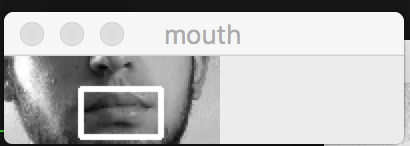
\includegraphics[width=0.25\textwidth]{./closd_mouth1.png}
\caption{Yawn detection: closed mouth}
\label{fig:noyawn}
\end{figure}
The resulting bounding box is shown in Figure \ref{fig:noyawn}. 
Similarly with the eye and face detection, we made use of built-in functionality of OpenCV's classification algorithms to identify a mouth. The OpenCV classification takes a wide array of parameters as inputs. A few of these parameters are listed:
\begin{itemize}
\item Min Size: minimum size of detected object (w,h). used = (20,20)
\item Min Neighbors: Parameter specifying how many neighbors each candidate rectangle should have to retain it. used = 4
\item Scale: Parameter identifying how much the image can be scaled for classification at each image frame (low values closer to 0 result in higher number of false positives). used=1.3
\end{itemize}
In order to correctly identify a yawn, we limited the bounding box to a very small area which is in line with our test subjects. This area limitation created a miss in mouth detection when an individual was yawning. This missed detection can be seen in Figure \ref{fig:yawn}, where the mouth goes past the limit of the bounding box and thus it is not recognized. 
\subsection{Blink Detection}

% \begin{wrapfigure}{L}{0.7\linewidth}
% 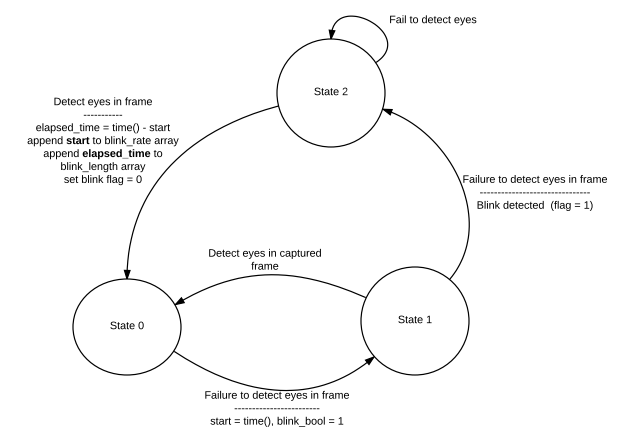
\includegraphics[width=\linewidth]{./state_machine_blink.png}
% \centering 
% \caption{State machine diagram for blink detection}
% \end{wrapfigure} 
As mentioned before, we proposed an algorithm that makes use of the image analysis techniques mentioned earlier within this section in order to detect the necessary features to classify the level of drowsiness that should generate an alert. The algorithm proposed to detect the blink rate and blink length is an implementation of a finite state machine which feeds its result to a historic data array, a portion of which is then analyzed and sent to the back-end storage. A discussion of the finite state machine follows: \\

\begin{figure}[H]
\centering
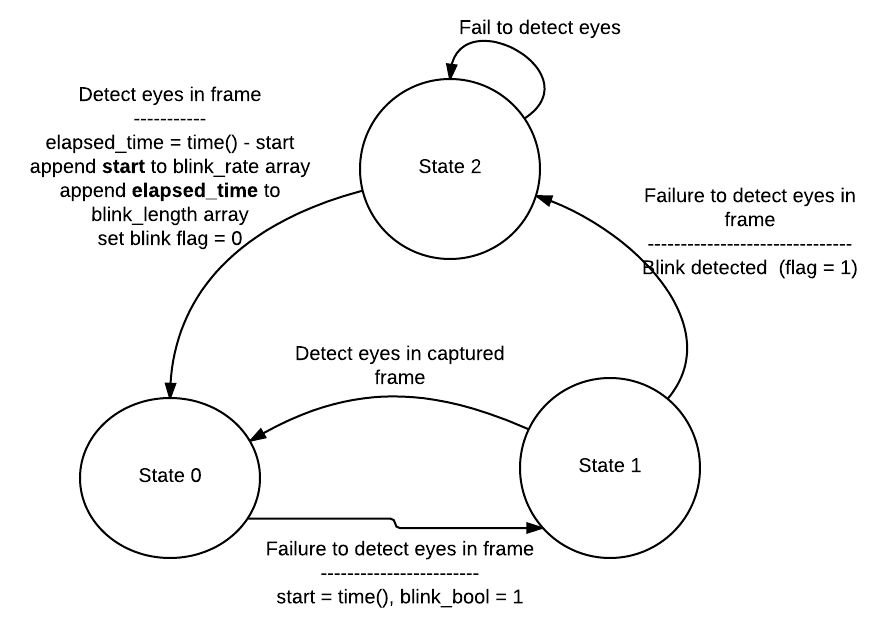
\includegraphics[width=1.1\linewidth]{./state_machine.png}
\caption{Blink Finite State Machine }
\label{fig:blink_fsm}
\end{figure}

The Finite state machine can be seen in Figure \ref{fig:blink_fsm}. Its operation spans a minimum of 3 frames, 2 to detect a blink and 3 to also detect the length of the blink. Using the Python time library allows reliable measurement of blink length without the need to account for different fps performance in the algorithm. After a blink is detected and its time and length calculated, that information is saved in two separate arrays. The array containing information about the start time of a blink is used to determine blink ratio (blinks per minute) whereas the blink length array is used to determine the average blink length. \\
The features used in the classification algorithm are as follows:
\begin{itemize}
\item Blink start time $\implies$ Append to array of blink start times $[b_0, b_1, b_2m\cdots]$
\item Blink length $\implies$ Append to array of blink lengths $[l_0,l_1,l_2,\cdots]$
\end{itemize}



\subsection{Yawn Detection}
The Yawn detection algorithm is very similar as the blink detection algorithm. The mouth detection proved to be less robust and more prone to misses, and thus we decided to have a threshold of minimum 5 continuous non-mouth frames to determine that a yawn was executed. Other considerations were taken into account to determine a yawn since there were many false positives while testing. False positives were triggered for anything from a person looking away, talking loudly, or placing a hand in front of the mouth. Further work on yawn detection could provide a more reliable drowsiness detection algorithm. 

\begin{figure}[H]
\centering
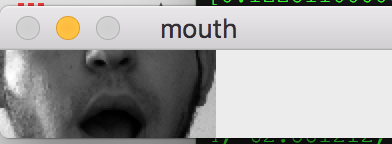
\includegraphics[width=0.25\textwidth]{./open_mouth.png}
\caption{Yawn detection: yawning}
\label{fig:yawn}
\end{figure}

\subsection{Threshold Calculation}
In order to determine whether the driver is sleepy or not, we collected samples from 20 individuals. To establish ground truth, we used a small questionnaire previous to the study and in addition, considered the time of day. \\
A classifier was trained using 169 negative data points and 123 positive data points from 20 individuals. The machine-learning tool Weka allows to compare multiple classification algorithms with the given data without having to code the algorithms. We tested variants of J48 decision trees, Random Forest, and Naive Bayes.  A discussion on the results of this classification task can be found in the results section. \\
The decisions of the drowsiness detection classification is performed every 20 seconds. The system uses the resulting J48 classification tree and performs a quick classification. Then, it forwards the data (current blink and yawn rate, as well as avg blink length and the threshold variable, which is set to 1 if the user is drowsy and 0 otherwise) via an HTTP Post request to the back-end server, where the data is stored. 

\section{Driver Alert Mechanism}
\begin{figure}
\centering
  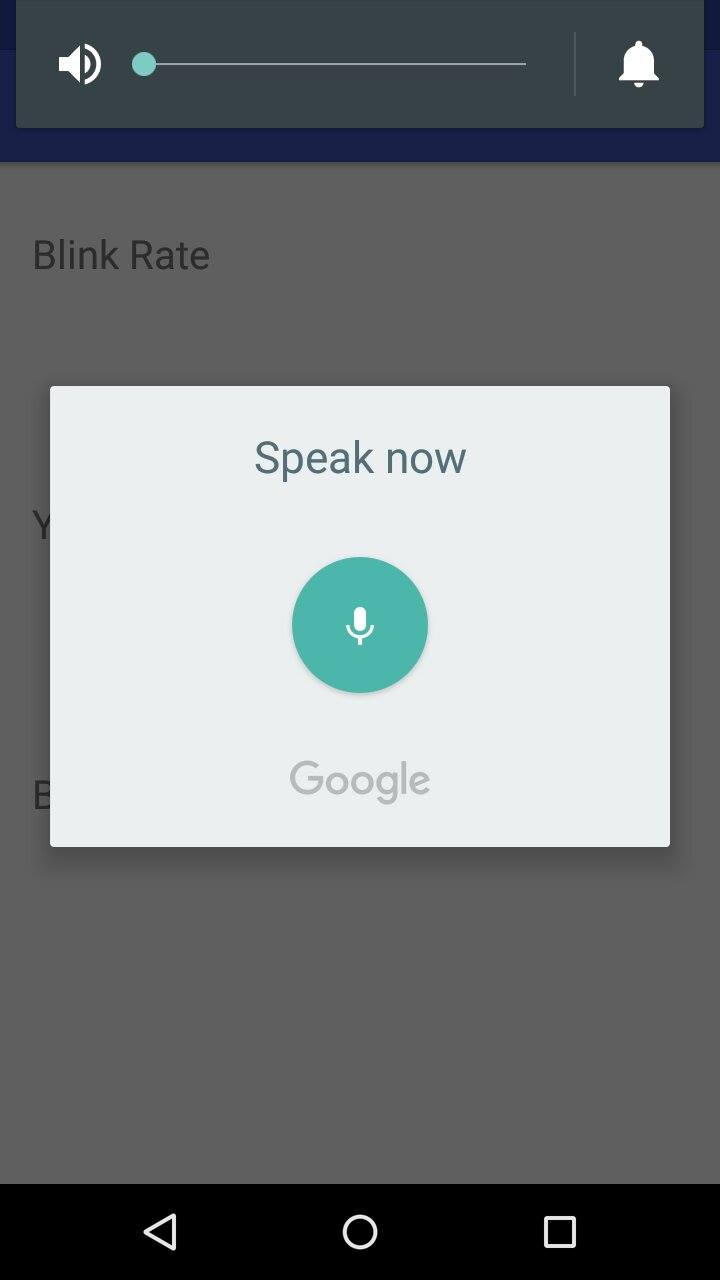
\includegraphics[width=.5\linewidth]{speaknow.jpg}
  \caption{Google voice recognition}
  \label{fig:voice}
\end{figure}

As data from the driver's face is collected and processed and a classification is made, the result is sent to the back-end server. The back-end server stores the information and saves it for when the mobile application retrieves the data. 
\subsection{Motivation}
We chose to have a driver alert mechanism which also incorporated a tangible solution because many available systems attempt to detect drowsy driving but do not provide proper feedback or an effective solution. Other systems ask for direct user interaction with the smarphone's touchscreen, which is dangerous since it requires the user to look away from the road. Most solutions found online included interaction with the phone in ways that can be dangerous and increase the probability of a crash. We propose a hands-free, voice-activated alert system. 
\subsection{Alert}
A smartphone submits a request directly to the back-end server. When the back-end server obtains the request, the response is sent in the form of a JSON file. Along with the most recent data on blink rate, blink length, and yawn rate, the data includes a threshold value which determines if the driver is sleepy or not. Upon the receipt of the proper threshold value indicating that the driver is drowsy, the smartphone activates the alert message. The alert message consists of a loud, easy to understand notification that could in the future be customized to the user's desire. Google's Text-To-Speech API was used in order to generate the alert. A typical alert would sound the following message: "Hey John, you seem sleepy. Do you want to get a coffee?" After a 5-second waiting period, voice recognition is triggered to ask for a response from the user.
\subsection{Voice Recognition}
The Voice Recognition system is shown in Figure \ref{fig:voice}. In the voice recognition phase, the system listens to the user's response to an alert message. A reply that is not strictly 'yes' will force the App to return to its normal state of near-real-time data collection. After a designated waiting time (5 seconds) it will request data again from the server and as long as the threshold is still active, it will prompt the user again with the same alert message and option to reply. A reply of 'yes' will trigger the Google Maps API. In order to recognize the human response, we made use of the Google Voice Recognition API, which returns a string of concatenated replies. As an example, saying "yes" would return a string similar to "yesyeahyeYESYesyepjees" Thus, we need only look if the desired feedback information 'yes' is contained within the resulting recognized string. 
\subsection{Maps}
\begin{figure}[H]
\centering
  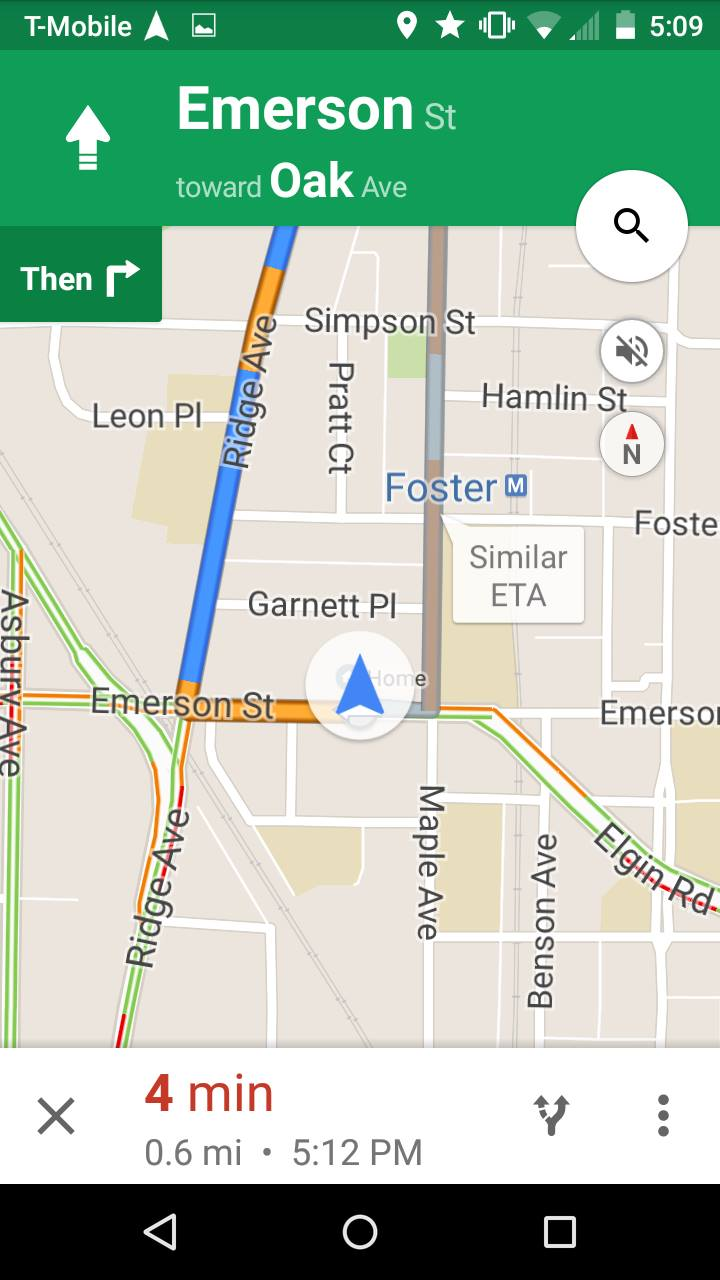
\includegraphics[width=.5\linewidth]{load_map.jpg}
  \caption{Maps integration}
  \label{fig:map}
\end{figure}

A reply of 'yes' triggers an event within the Android phone that connects directly with the Google Maps app, as seen in Figure \ref{fig:map}. The motivation to use the Google Maps app was to provide a real and effective solution. One of the related studies \cite{pakistan} does not take action once drowsiness has been detected, and thus successfully identifies the problem but does not provide a feasible and safe solution. 

\section{Experimental Set Up and Testing}
Because of the inherent danger of running a clinical trial on real drowsy subjects driving a car, testing was done in a safe and quiet environment.  The first step in order to build the classifier was to gather data from individuals in order to create a classification algorithm. Data from 20 individuals was captured using various devices, including both a Macbook Pro and a Raspberry Pi with an attached camera module. A Macbook Pro was used in order to provide faster, more detailed time-series data than a Raspberry Pi.  \\
In order to test how robust the system is to different factors, some tests were made by people wearing clear glasses and some by people without glasses. Additionally, some tests were made with improper lighting conditions: a shaded area and a quickly changing shadows that covered the face at irregular periods of time. The results determined that clear glasses with thin or non-existent frames did not affect the eye identification, while thick frames increased the error rate. Needless to say, this system would not work when a driver is wearing sunglasses. 
It should be noted that blink detection requires at least 2 subsequent frames of failed eye detection. Considering that the average human blinks for $200-400$ milliseconds, there is a minimum performance requirement. The minimum FPS calculation is as follows:
$$FPS_{min} = 2*(1/.2) = 10 FPS$$ 
This measurement is for the lower end of the average human blink. When testing the design, we noticed that this average was in fact true, and thus any implementation that did not manage to achieve a minimum of 10 FPS performance would render wrong results due to missed frames. \\

\section{Results and Discussion}
\subsection{Data Analysis}
We analyzed the data collection results and the performance of our algorithm. Additionally, we tested the functionality of the system as a whole. 
% show the features as results 
\begin{figure}[H]
\centering
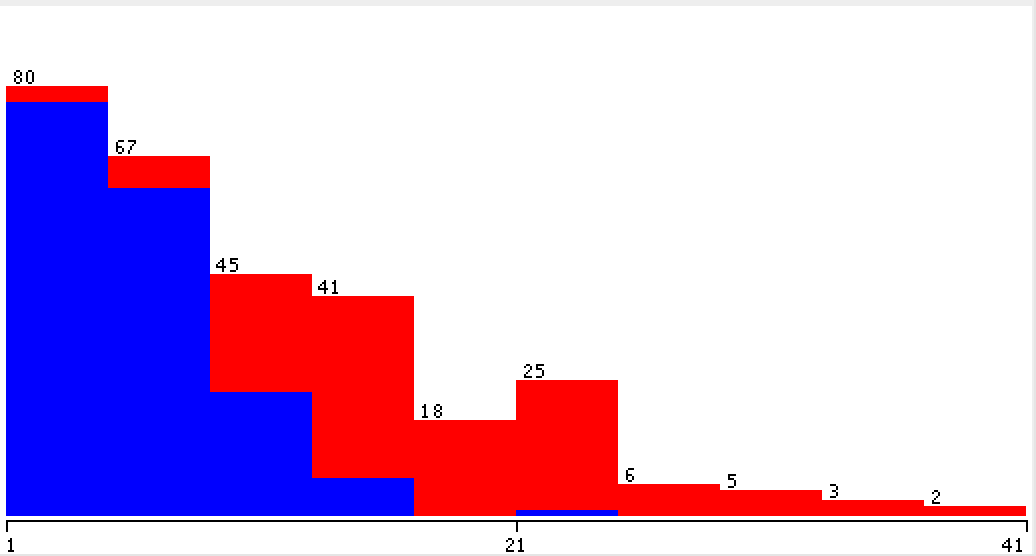
\includegraphics[width=0.8\linewidth]{./blink_rate.png}
\caption{Blink Rate Histogram }
\label{fig:blink_hist}
\end{figure}

Figure \ref{fig:blink_hist} shows a histogram of the blink rate (average blinks per minute) from the collected data. Note that red represents the positive state (drowsy) and blue represents the negative state (not drowsy). When performing feature selection, it was easy to see that blink rate was the most important feature in the classification task. 

\begin{figure}[H]
\centering
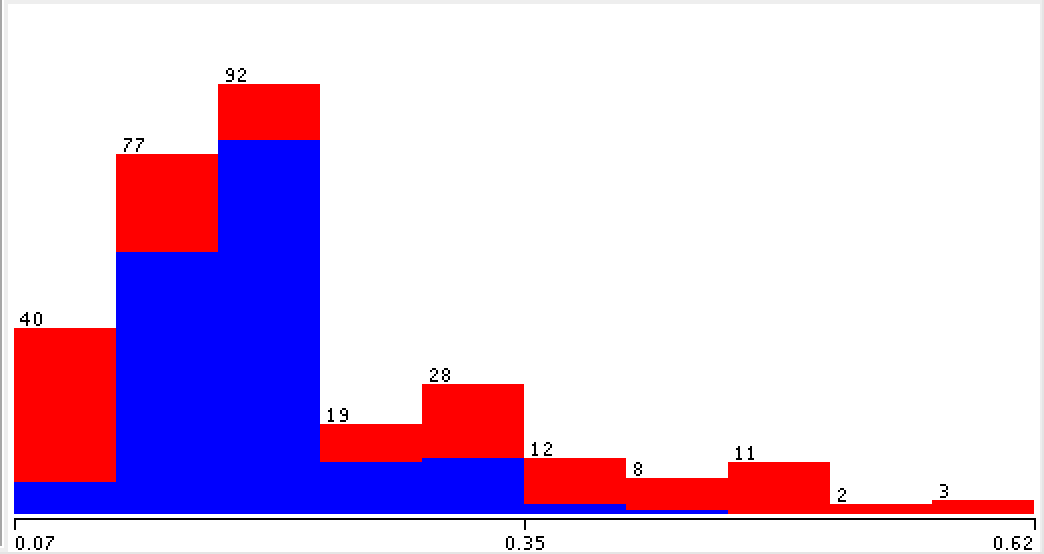
\includegraphics[width=0.8\linewidth]{./blink_length.png}
\caption{Blink Length Histogram }
\label{fig:blink_length_hist}
\end{figure}


Figure \ref{fig:blink_length_hist} shows the blink length histogram, that is the distribution of blink length for the sampled data. It should be noted that this is not as robust of a feature, since there is a large portion of blinks of a minimum length where the classification is drowsy. Finally, Figure \ref{fig:yawn_hist} shows the distribution of the yawn rate in our tests. Even though this histogram seems skewed towards 0 yawn per minute, it is a reasonable measurement since most non-drowsy people will not yawn in a relatively long period of time. 

\begin{figure}[H]
\centering
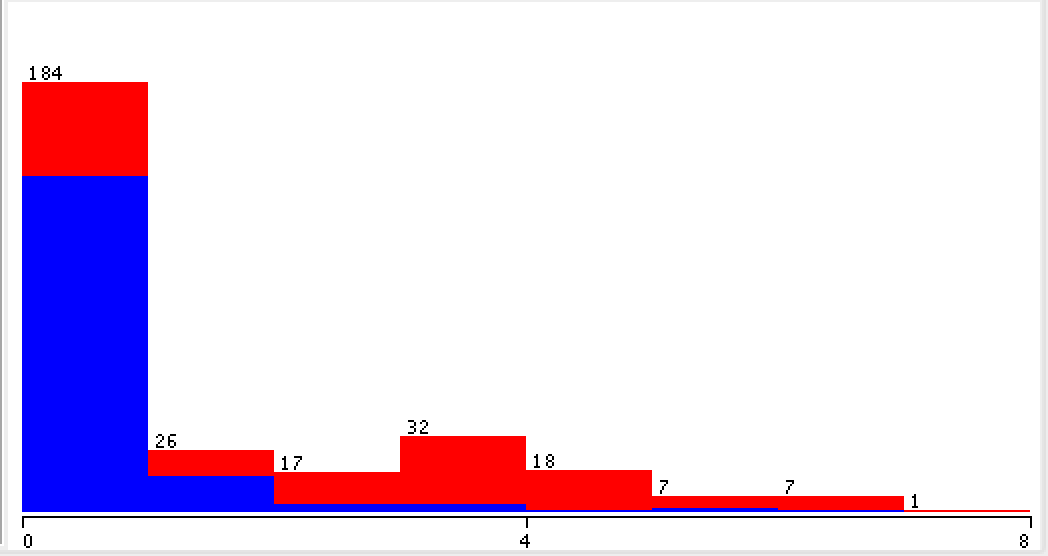
\includegraphics[width=0.8\linewidth]{./yawn_rate.png}
\caption{Yawn Rate Histogram }
\label{fig:yawn_hist}
\end{figure}

\subsection{Algorithm Performance}

Because of the computationally heavy nature of the algorithm, we tested our implementation in different hardware. We tested different implementations in which we varied the image size and the hardware used. Table \ref{tab:results_1} shows the performance in Frames Per Second for each of the implementations. As mentioned previously, a frame rate lower than 10 FPS renders a very weak blink detection algorithm and thus cannot be considered reliable for drowsiness detection. This renders our Raspberry Pi implementation too slow to be useful. Further optimization of the algorithm, changes in design, multi-threading, and the newer version of the Raspberry Pi - the Raspberry Pi 3 -  are all factors that could help increase efficiency and create a working mobile solution. \\
\medskip 
Another consideration of this algorithm is its effectiveness to perform under different lighting conditions. Upon testing, we noticed that as soon as a large shadow covered the eye region and not the rest of the frame, blink detection began to fail. Since eyes were detected fewer times than under normal lighting conditions, the blink ratio increased. Attempts at eliminating this issue includes minimum blink detection, where a blink would not only needs 2 frames but also 100 milliseconds in order to be counted as a valid blink. 

\begin{table}[H]
\centering
\begin{tabular}{l|c|r}
Implementation & Image Capture Size & FPS \\\hline
MacBook Pro 2014 &(640,800) & 18 \\
MacBook Pro 2012 &(640,800) & 17 \\
Raspberry Pi & (640,800) & 4 \\
Raspberry Pi & (300,400) & 6
\end{tabular}
\caption{\label{tab:results_1}Classification algorithms}
\end{table}

\subsection{Machine Learning - Classification}

The classification algorithm was created with the aid of Weka. Table \ref{tab:algo_compare} shows the different results of each algorithm after performing 10-fold cross validation on the dataset. The dataset had 292 total instances.  

\begin{table}[H]
\centering
\begin{tabular}{l|c|c|r}
Classifier & \% Correct & Precision & Recall \\\hline
J48 & 90.06\% & 0.901 & 0.901 \\
Naive Bayes & 93.15\% & 0.932 & 0.932 \\
Random Forest & 92.46\% & 0.925 & 0.925
\end{tabular}
\caption{\label{tab:algo_compare}Performance results}
\end{table}

As shown in Table \ref{tab:algo_compare}, all algorithms showed at least 90\% correct classification. For simplicity, the J48 decision tree was implemented in the Python script that determined the drowsiness classification. The confusion matrix for the J48 classification is shown in Table \ref{tab:confusion}. 
\begin{table}[H]
\centering
\begin{tabular}{l|c|r}
.& Non-drowsy & Drowsy  \\\hline
Classified = Non-drowsy & 158 & 11 \\
Classified = drowsy & 11 & 112 
\end{tabular}
\caption{\label{tab:confusion}Confusion Matrix for J48 classification}
\end{table}


\section{Conclusion and Future Work}
We proposed a new efficient drowsiness detection for real-time implementation by making use of blink and yawn detection. This techniques gives accurate results when subjected to the proper lighting conditions and with enough processing power. We also successfully tested the software on people wearing glasses with no discernible change.\\
Future work on developing this application would account for people wearing headwear, or who have any physiological properties that prevents a face, eye, or mouth from being recognized. In addition, an increased input from AI technologies and Machine Learning would allow the system to learn individual blinking patterns, driving behavior, etc and build a personalized drowsiness detection that can be customized in order to improve accuracy. \\
Performance improvements would allow this system to be mounted on a small, portable computer such as the Raspberry Pi without having to re-engineer the entire system. The newest Pi, the Raspberry Pi 3, is equipped with larger processing power and could potentially be used in this project. Moving some of the code-base to C or C++ could also prove very beneficial for efficiency purposes. 


\begin{thebibliography}{1}

  \bibitem{norman} E. H. Norman {\em Japan's emergence as a modern
  state} 1940: International Secretariat, Institute of Pacific
  Relations.

  \bibitem{viola}P. Viola and M. Jones, "Rapid object detection using a boosted cascade of simple features," Computer Vision and Pattern Recognition, 2001. CVPR 2001. Proceedings of the 2001 IEEE Computer Society Conference on, 2001, pp. I-511-I-518 vol.1.
  
  \bibitem{fusion} B.-G. Lee and W.-Y. Chung, “Driver Alertness Monitoring Using Fusion of Facial Features and Bio-Signals,” IEEE Sensors Journal, vol. 12, no. 7, pp. 2416–2422, Jul. 2012.
  
  \bibitem{sultan} S. Al-Sultan, A. Al-Bayatti, and H. Zedan, “Context Aware Driver Behaviour Detection System in Intelligent Transportation Systems (ITS).,” IEEE Transactions on Vehicular Technology, no. c, pp. 1–1, 2013.

   \bibitem{braincomputer} Chin-Teng Lin, Che-Jui Chang, Bor-Shyh Lin, Shao-Hang Hung, Chih-Feng Chao, and I-Jan Wang, “A real-time wireless braincomputer interface system for drowsiness detection.,” IEEE transactions on biomedical circuits and systems, vol. 4, no. 4, pp. 214–22, Aug. 2010.

	\bibitem{eeg_fuzzy} ] C. Lin, Y. Chen, R. Wu, S. Liang, and T. Huang, “Assessment of Driver’s Driving Performance and Alertness Using EEG-based Fuzzy Neural Networks,” 2005 IEEE International Symposium on Circuits and Systems, pp. 152–155, 2005.

	\bibitem{eeg_spectrum} D. Kim, H. Han, S. Cho, and U. Chong, “Detection of Drowsiness with eyes open using EEG- Based Power Spectrum Analysis,” 2012 7th International Forum on Strategic Technology (IFOST), Tomsk, pp. 3–6, 2013.

	\bibitem{driving_manuever} A. Sathyanarayana, S. O. Sadjadi, and J. H. L. Hansen, “Leveraging sensor information from portable devices towards automatic driving maneuver recognition,” 2012 15th International IEEE Conference on Intelligent Transportation Systems, pp. 660–665, Sep. 2012.
	\bibitem{sleep_depravation} L. Tijerina, T. Pilutti, J. F. Coughlin, and E. Feron, “Detection of Driver Fatigue Caused by Sleep Deprivation,” IEEE Transactions on Systems, Man, and Cybernetics - Part A: Systems and Humans, vol. 39, no. 4, pp. 694–705, Jul. 2009.

	\bibitem{pascale} A. Pascale, M. Nicoli, F. Deflorio, B. Dalla Chiara, and U. Spagnolini, “Wireless sensor networks for traffic management and road safety,” IET Intelligent Transport Systems, vol. 6, no. 1, p. 67, 2012.
    
    \bibitem{smartcar} J. Sun, Y. Zhang, and K. He, “Providing Context-awareness in the Smart Car Environment,” 2010 10th IEEE International Conference on Computer and Information Technology, no. Cit, pp. 13–19, Jun. 2010.

	\bibitem{pakistan}A. Rahman, M. Sirshar and A. Khan, "Real time drowsiness detection using eye blink monitoring," 2015 National Software Engineering Conference (NSEC), Rawalpindi, 2015, pp. 1-7.
doi: 10.1109/NSEC.2015.7396336

  \end{thebibliography}


\end{document}
